\chapter{Konzeption des Systems}
\label{chap:konzeption}

Die Konzeption des Systems bildet das Fundament für die spätere Implementierung und vereint moderne Technologien, um eine leistungsfähige und benutzerfreundliche Mitarbeitergesprächssoftware zu entwickeln. Im Zentrum der Konzeption stehen drei essenzielle Bereiche: das Design, die technischen Komponenten und die Datenarchitektur.

Das System zielt darauf ab, durch die Kombination von Frontend-Technologien wie React und Vite mit einem effizienten Backend auf Basis von .NET Core eine skalierbare und zuverlässige Plattform zu schaffen \cite{kirk2016data, microsoftDotNet}. Ergänzt wird dies durch eine relationale Datenbankstruktur, die mit Azure SQL realisiert wird, um eine robuste und sichere Speicherung sowie Verarbeitung der Gesprächsdaten zu gewährleisten \cite{azureDocumentation}.

Ein besonderer Fokus liegt auf der Interoperabilität mit bestehenden HR-Infrastrukturen. Durch den Einsatz von Microsoft Azure-Diensten wie Active Directory und Microsoft Graph wird eine nahtlose Integration ermöglicht, die nicht nur die Benutzerfreundlichkeit steigert, sondern auch die Effizienz datenbasierter Entscheidungsprozesse fördert \cite{microsoftAzure}. Die Architektur ist darauf ausgelegt, Visualisierungstools wie Donut- und Radarcharts zu integrieren, die eine intuitive und präzise Darstellung komplexer Daten unterstützen \cite{evergreen2016effective}.

Diese Konzeption stellt sicher, dass die verschiedenen Komponenten des Systems harmonisch zusammenwirken, um den Anforderungen moderner Arbeitsumgebungen gerecht zu werden und gleichzeitig die Grundlage für eine zukunftssichere Weiterentwicklung zu schaffen.

\section{Frontend-Architektur}
Das Frontend des Systems wird mit React und Vite geplant, um eine hohe Performance und schnelle Entwicklungszyklen zu gewährleisten. React dient als Kerntechnologie für die komponentenbasierte Architektur \cite{facebook2021react}, während Vite als moderner Build-Toolchain für eine optimale Ladezeit und Hot-Module-Replacement vorgesehen ist \cite{vite2022docs}. Zur Sicherstellung der Codequalität und Einhaltung von Best Practices wird ESLint integriert, um den Code auf potenzielle Fehler und Stilabweichungen zu überprüfen \cite{eslint2022guide}. Dies gewährleistet eine konsistente und wartbare Codebasis während der gesamten Entwicklungsphase.

\subsubsection*{Technische Grundlagen und Implementierung}
Das Frontend wird mit TypeScript geplant, um durch statische Typisierung die Lesbarkeit und Wartbarkeit des Codes zu erhöhen. Die Wahl der Technologien und Bibliotheken erfolgt gezielt, um die spezifischen Anforderungen des Projekts hinsichtlich Skalierbarkeit, Sicherheit und Benutzerfreundlichkeit zu erfüllen.

HTML bildet die Grundlage für die Strukturierung der Inhalte auf der Benutzeroberfläche, da es eine bewährte Basis für moderne Frameworks wie React bietet. React und react-dom werden für ihre komponentenbasierte Architektur gewählt, die eine effiziente Wiederverwendbarkeit von UI-Elementen ermöglicht \cite{facebook2021react}. 

Für das State-Management werden Redux Toolkit und Zustand evaluiert. Redux Toolkit wird für komplexere Datenflüsse verwendet, während Zustand aufgrund seiner Einfachheit für fokussierte Zustände gewählt wird. Zur Darstellung von Daten wird die Bibliothek ApexCharts geplant, da sie interaktive Diagramme wie Donut- und Radarcharts unterstützt \cite{apexchartsDoc}. 

\subsubsection*{Prototyping und Benutzerzentrierung} 
Für das Prototyping wird Figma verwendet, um frühzeitig Feedback zur Benutzeroberfläche einzuholen und diese iterativ zu verbessern. Dieser Ansatz sichert eine benutzerzentrierte Entwicklung, die den Anforderungen der Zielgruppe entspricht.

\subsubsection*{Entwicklungsprozesse und DevOps} 
Das Projekt wird mittels Azure Pipelines in eine CI/CD-Pipeline integriert. Dies ermöglicht automatisierte Tests und Deployments des Frontends in verschiedene Umgebungen. Zudem wird Docker für die Containerisierung genutzt, um eine konsistente Entwicklungs- und Produktionsumgebung sicherzustellen.

\section{Backend-Architektur}
Die Backend-Architektur stellt eine zentrale Komponente in der Planungsphase des Systems dar und soll eine robuste und skalierbare Grundlage für die Verarbeitung und Speicherung der Daten bieten. Verschiedene Technologien und Ansätze wurden evaluiert, um die effizienteste Lösung für die Anforderungen des Projekts zu identifizieren.

\subsubsection*{Zentrale Dienste und Technologien}
Die geplante Backend-Architektur basiert auf einer modularen Struktur, die mehrere essenzielle Dienste und Technologien integriert. Der Azure Service Bus wird für die Verarbeitung und Synchronisation von Nachrichten zwischen den verschiedenen Systemkomponenten vorgesehen. Das Publish-Subscribe-Muster reduziert die Kopplung zwischen Systemkomponenten und ermöglicht eine flexible Integration neuer Komponenten sowie eine hohe Skalierbarkeit \cite{azureServiceBus2024}.

Für den Datenbankzugriff wird Entity Framework Core evaluiert, das im Vergleich zu Tools wie Dapper eine höhere Abstraktionsebene und nahtlose Integration mit .NET Core bietet \cite{entityFrameworkCore2020}. Zusätzlich werden Hintergrundjobs für automatisierte Aufgaben wie das Versenden von Benachrichtigungen oder das Berechnen aggregierter Daten entworfen \cite{backgroundTasks2017}.

\subsubsection*{Technologien und Abhängigkeiten}
Zu den geplanten Abhängigkeiten zählen:
- AutoMapper für die Abbildung von Datenmodellen \cite{automapperDocs2024}.
- MassTransit und MassTransit.Azure.ServiceBus.Core für Messaging-Lösungen \cite{masstransit2021}.
- Microsoft.Identity.Web zur Integration von Azure Active Directory.

Durch diese sorgfältige Planung wird eine flexible, sichere und skalierbare Backend-Architektur geschaffen.

\section{Datenbankdesign}
Die Konzeption der Datenbank ist ein zentraler Bestandteil der Systemplanung, da sie das Rückgrat für die Speicherung und Verarbeitung großer Datenmengen bildet. Nach der Prüfung von PostgreSQL und MySQL fiel die Entscheidung auf Microsoft SQL Server, da es eine nahtlose Integration mit Azure-Diensten und umfangreiche Sicherheitsfunktionen bietet.

\subsubsection*{Sicherheitsmaßnahmen}
Die Datenbank soll durch Verschlüsselung und rollenspezifische Zugriffsrechte geschützt werden, um Datenschutzrichtlinien wie die DSGVO zu erfüllen \cite{liu2021security}.

\subsection{Datenbankstruktur}
Die geplante Datenbankstruktur umfasst Tabellen wie \textbf{EmployeeAppraisal} für Gesprächsdaten und \textbf{AppraisalGroup} für Gruppierungen. Ziel ist eine klare Organisation und Vermeidung redundanter Daten.

\subsection{Beziehungsmodell}
Die geplante Datenbank folgt einem relationalen Modell, das effiziente Abfragen ermöglicht. Abbildung \ref{fig:db_er_model} zeigt das ER-Diagramm der geplanten Datenbankstruktur.

\begin{figure}[h!]
    \centering
    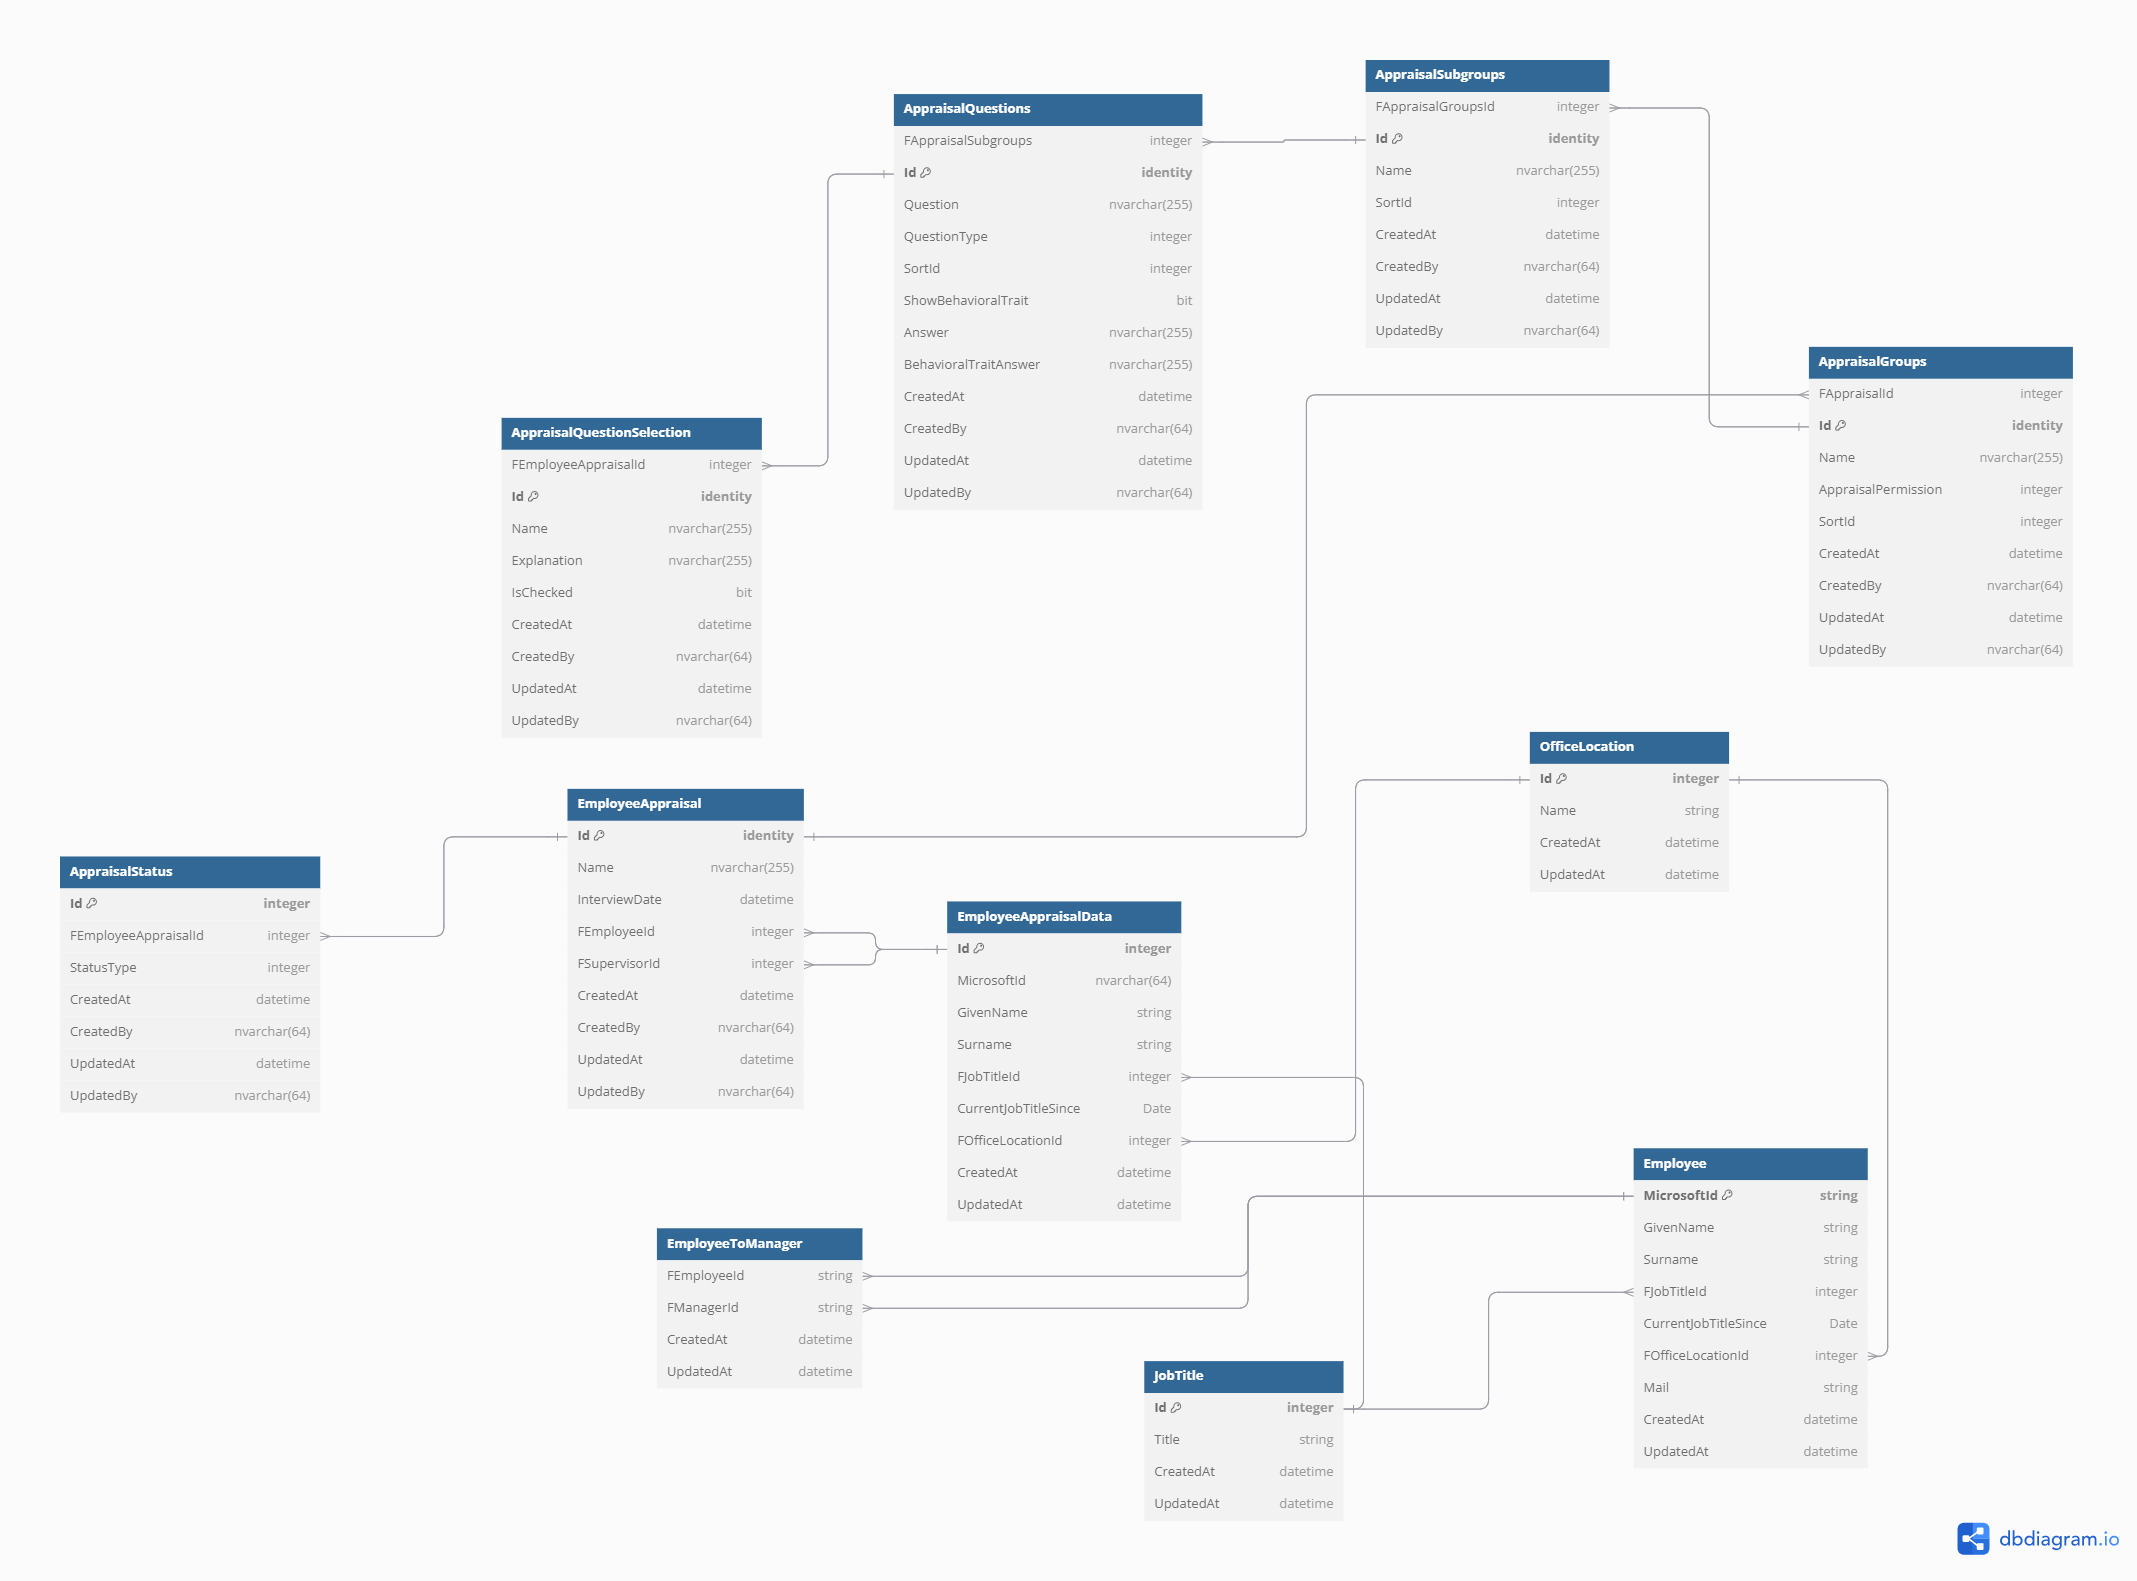
\includegraphics[width=1.0\textwidth]{images/er_modell_design.png}
    \caption{ER-Diagramm der geplanten Datenbankstruktur.}
    \label{fig:db_er_model}
\end{figure}

\section{Workflows}
Für die Nachrichtenverarbeitung wird der Azure Service Bus evaluiert, während für geplante Hintergrundjobs Hangfire als bevorzugte Lösung vorgesehen ist. Ziel ist eine flexible und skalierbare Systemkommunikation.

\section{Sicherheitskonzepte}
Die Sicherheit des Systems wird durch Maßnahmen wie JWT-Authentifizierung, Verschlüsselung und rollenspezifische Zugriffskontrollen gewährleistet. Diese Sicherheitsmaßnahmen sollen die Integrität und Vertraulichkeit der Daten sicherstellen und den Anforderungen an moderne Unternehmensanwendungen gerecht werden.
